Der Lernfortschritt von Klassifikatoren besteht darin, besser in der Aussage zu werden, ob ein Label $y$ auf einen gegebenen Eingang $x$ zutrifft. Dafür benötigen sie annotierte Trainingsdaten. Schachalgorithmen sollen hingegen lernen, Züge zu spielen, die die Gewinnchancen des Algorithmus maximieren. Eine weitere Art von \acp{KNN} sind \emph{generative Netze}. Sie sollen lernen, neue Daten zu erzeugen, die der Verteilung der Trainingsdaten ähneln. Generative Netze zur Bildgenerierung sollen demnach anhand eines Trainingsdatensatzes lernen, welche Bilder sie erzeugen sollen. Dies lernen sie anhand der statistischen Verteilung der Trainingsdaten. Die Daten sind nicht annotiert, wodurch generative Netze in der Regel in das \emph{Unüberwachte Lernen} einzuordnen sind.

\subsection{Mathematischer Hintergrund}
Generative Netze zur Bilderzeugung sollen beurteilen können, wie wahrscheinlich es ist, dass ein gegebenes Bild aus der Verteilung der Trainingsdaten stammt. Wenn $x$ für jedes mögliche existierende Bild steht, so bilden generative Netze folgende Wahrscheinlichkeitsverteilung ab:
\begin{equation}
   \hat{p}(x)
\end{equation}
Für ein gegebenes Bild $x$ gibt $\hat{p}(x)$ einen Schätzwert dafür an, wie wahrscheinlich es ist, dass das Bild aus den Trainingsdaten stammt. Diese Wahrscheinlichkeitsverteilung wird durch das Netz erlernt. Optimiert wird, dass die geschätzte Verteilung der Daten $\hat{p}(x)$ möglichst ähnlich zu der tatsächlichen Verteilung der Trainingsdaten $p(x)$ ist. Ein beispielhafter Vergleich ist in Abbildung \ref{fig:generativeNetsPx} dargestellt. Es ist erkennbar, dass sich die geschätzte und die tatsächliche Verteilung ähnlich sehen, jedoch nicht identisch sind. Die Abweichung zwischen diesen Verteilungen stellt dabei die Kosten (engl.: den \emph{loss}) dar. Die schwarzen Punkte kennzeichnen Trainingsdaten. Durch sie soll die Verteilung $p(x)$ abgebildet werden. Weniger diversifizierte Trainingsdaten würden sich beispielsweise nur in einem Teilbereich von $p(x)$ befinden. Dadurch könnte das Modell $p(x)$ weniger gut approximieren.

\begin{figure}[H]
   \centering
   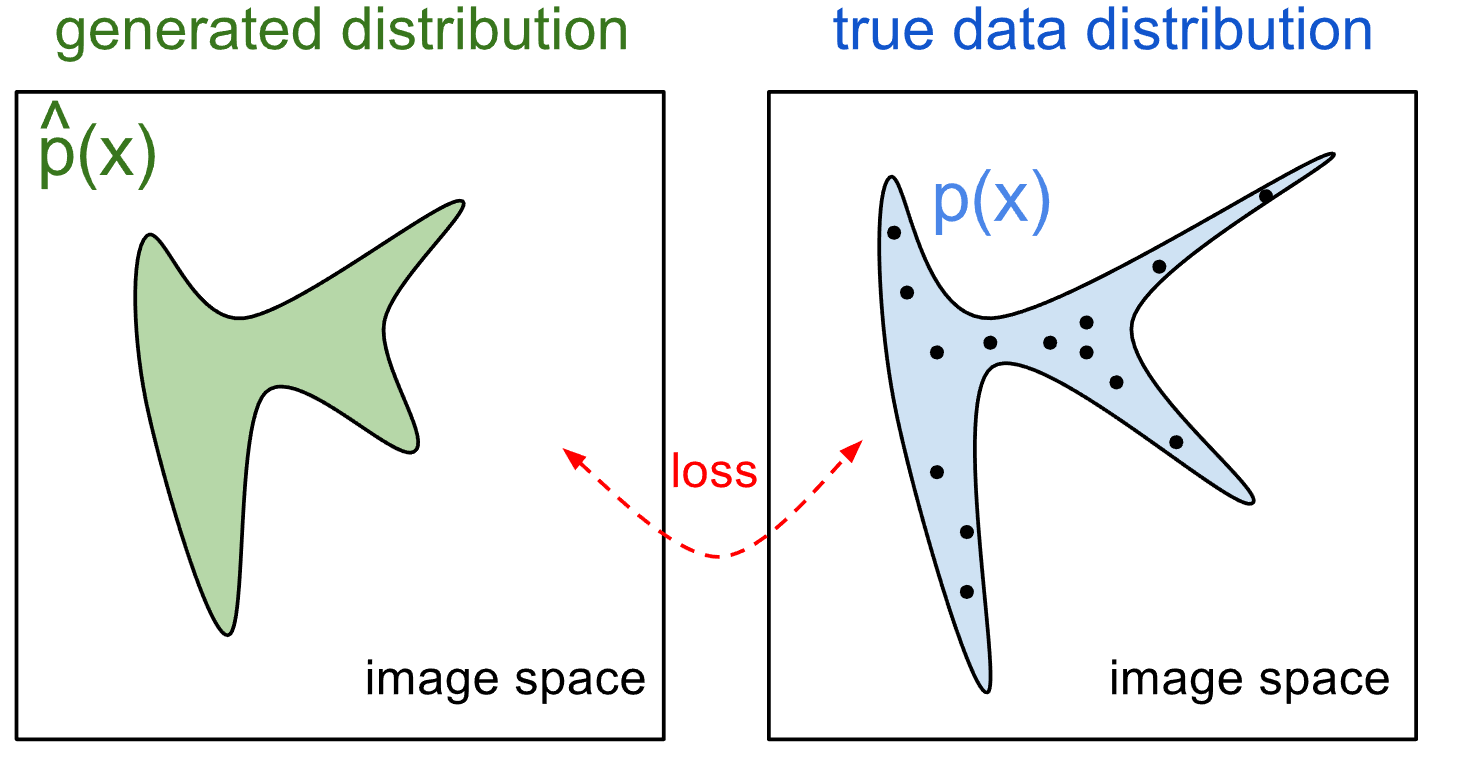
\includegraphics[width=0.5\textwidth]{images/Generative Networks/p(x) Distribution.png}
   \caption{Beispielhafter Vergleich von $\hat{p}(x)$ und $p(x)$ \cite{openAiGenerativeNets}}
   \label{fig:generativeNetsPx}
\end{figure}

Bei der Bildgenerierung versucht das Netz den Wahrscheinlichkeitswert für $\hat{p}(x)$ zu maximieren. Es erlernt durch $\hat{p}(x)$, wie die Verteilung der Trainingsdaten aussieht und versucht anschließend ausschließlich Bilder zu generieren, die dieser Verteilung folgen. Bezogen auf Abbildung \ref{fig:generativeNetsPx} befinden sich alle generierten Bilder des trainierten Netzes im grün markierten Bereich.

Es existieren verschiedene Arten generativer Netze. Die Taxonomie, also die Einteilung verschiedener Netze in bestimmte Kategorien, kann Abbildung \ref{fig:generativeModelsTaxonomy} entnommen werden. Einerseits existieren Architekturen, die die Wahrscheinlichkeitsverteilung $\hat{p}(x)$ explizit berechnen. Andere berechnen die Funktion nicht, verwenden sie jedoch implizit. In der Abbildung wird dahingehend zwischen \emph{Explicit Density Models} \emph{(explizit berechnete Dichte)} und \emph{Implicit Density Models} \emph{(implizit berechnete Dichte)} unterschieden. Es existieren zudem Unterkategorien, mittels derer eine feinere Kategorisierung durchgeführt wird.

\begin{figure}[H]
   \centering
   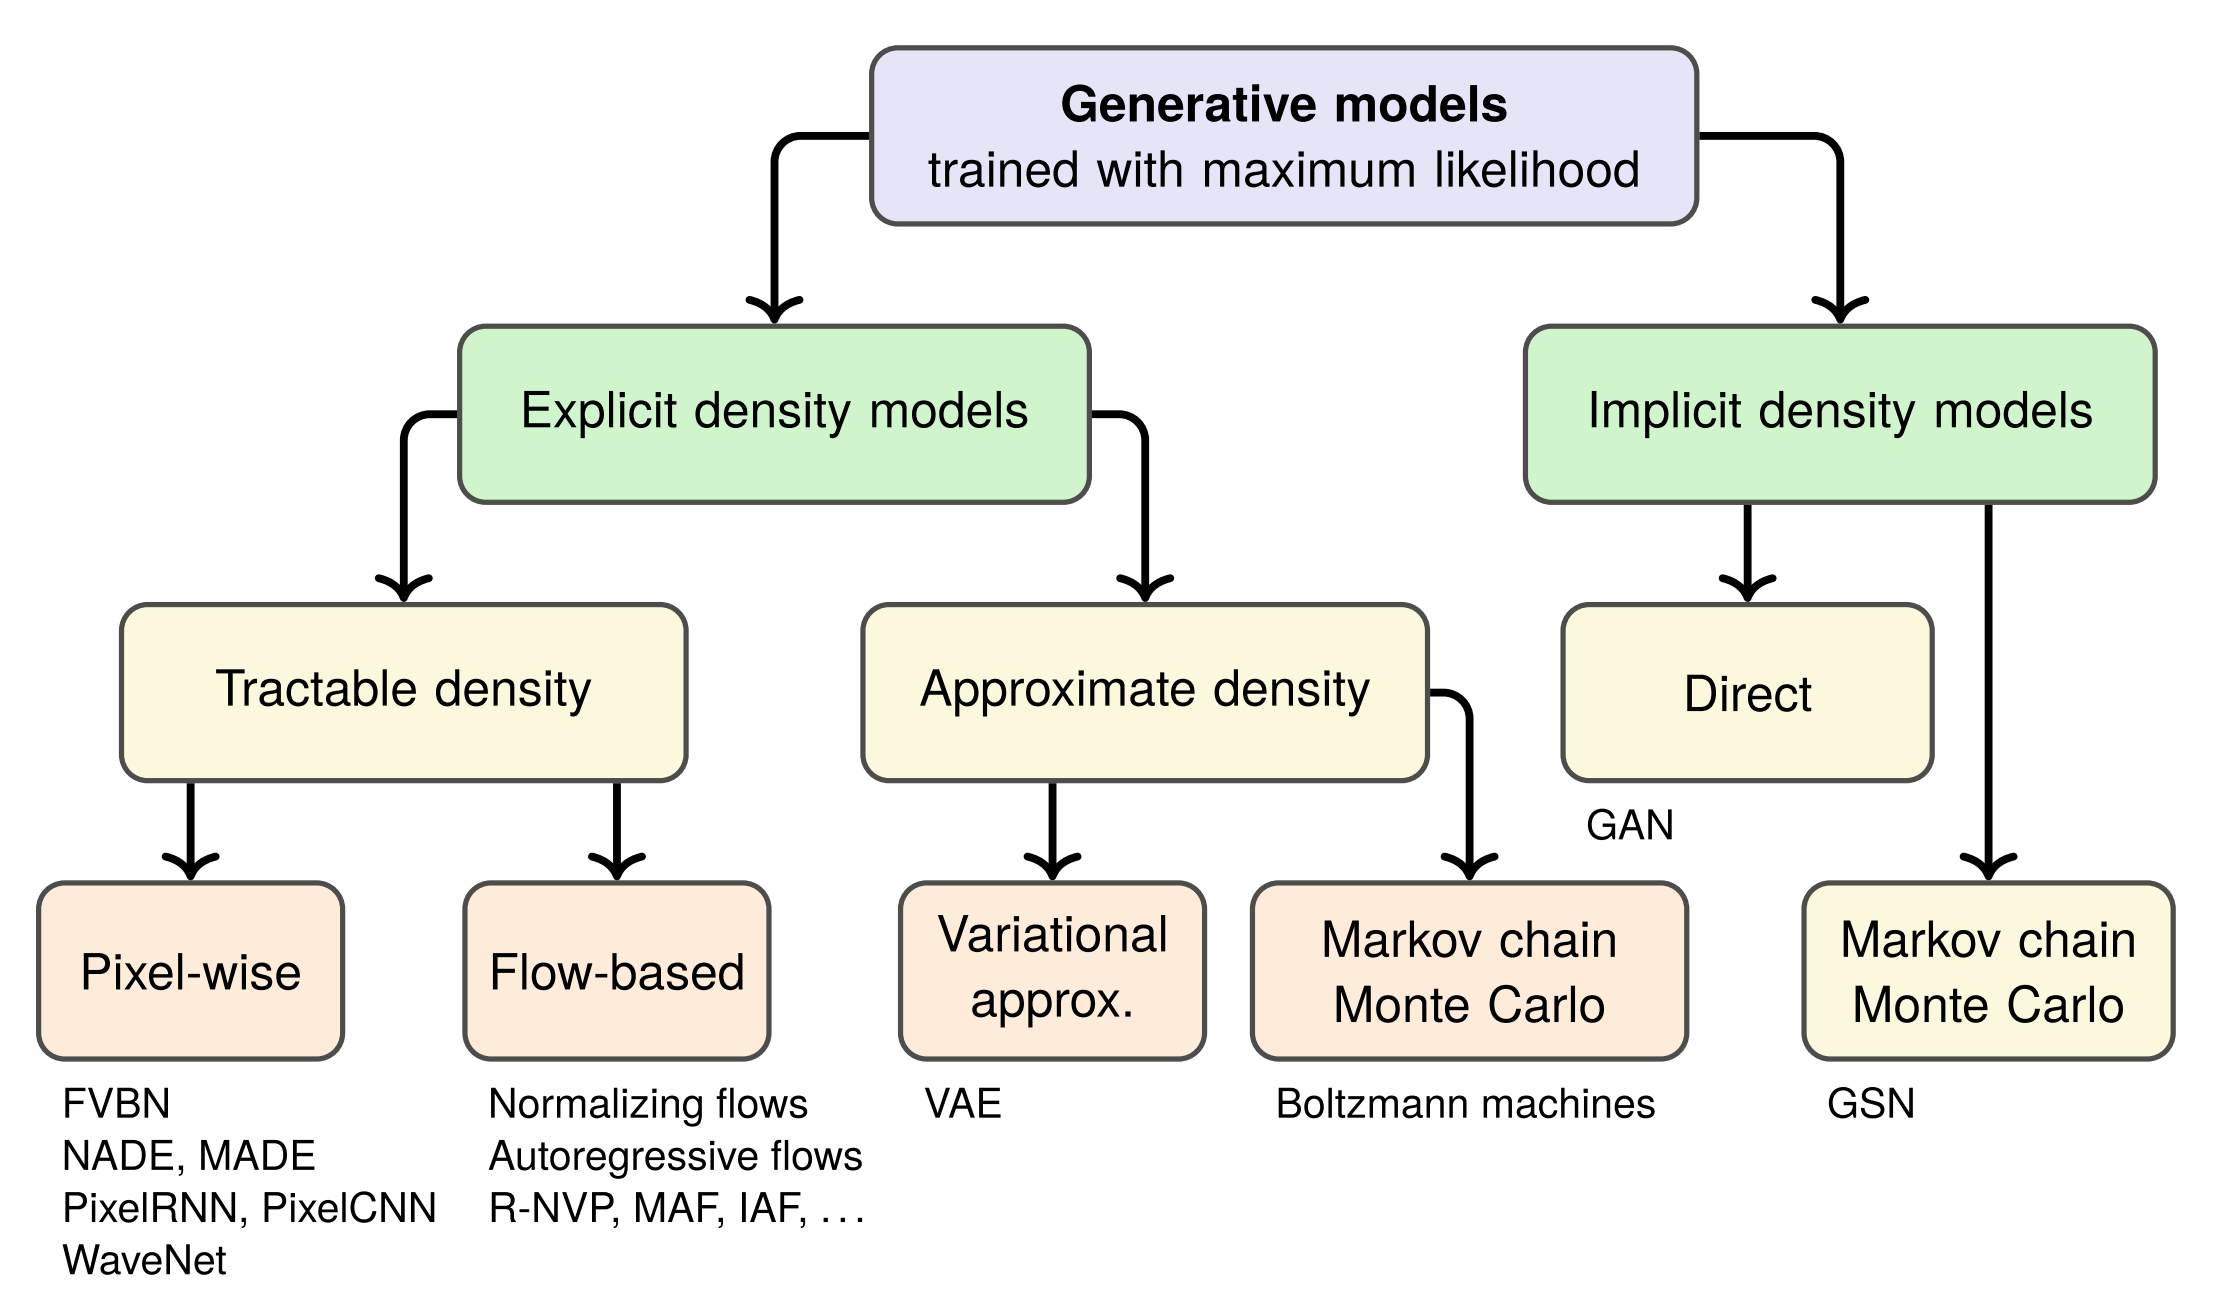
\includegraphics[width=0.8\textwidth]{images/Generative Networks/Taxonomy of Generative Models.png}
   \caption{Taxonomie generativer Modelle \cite{generativeModelsBook}}
   \label{fig:generativeModelsTaxonomy}
\end{figure}

Es soll in diesem Kapitel auf verschiene Architekturen generativer Netze eingegangen werden. \acp{GAN} werden gesondert in Kapitel \ref{chap:GANs} beschrieben.

\subsection{Pixel Recurrent Neural Networks}
Die Architektur der \acp{PixelRNN} stammt aus dem Jahr 2016. Diese Netze stützen sich explizit auf die Maximierung der Maximum-Likelihood-Schätzung von $\hat{p}(x)$ für jeden Pixel. Sie sind in der genannten Taxonomie den Modellen zuzuordnen, die den tatsächlichen Schätzwert von $p(x)$ berechnen können. \cite{pixelRNN}

Im folgenden soll geklärt werden, wie der optimale Wert für jeden Pixel eines generierten Bildes bestimmt wird. Ein betrachtetes Bild $x$ der Auflösung $n \times n$ kann in seine einzelnen Pixel $(x_{1}, x_{2}, ..., x_{n^2})$ aufgeteilt werden. In Gleichung \ref{eq-max-likelihood} ist dabei dargestellt, wie die Wahrscheinlichkeit eines jeden Pixels in die gesamte Verteilung $\hat{p}(x)$ einfließt. \cite{pixelRNN}
\begin{equation}
   \label{eq-max-likelihood}
   \hat{p}(x) = \hat{p}(x_{1}, x_{2}, ..., x_{n^2}) = \prod_{i=1}^{n^2}\hat{p}(x_{i}|x_{1},...,x_{i-1})
\end{equation}
Jeder Pixel $x_{i}$ besitzt eine eigene Wahrscheinlichkeitsverteilung $\hat{p}(x_{i}|x_{1},...,x_{i-1})$. Sie ist abhängig von allen anderen Pixeln $x_{1},...,x_{i-1}$ des Bildes. Der absolut optimale Wert eines Pixels kann demnach nur dann berechnet werden, wenn die Werte aller anderen Pixel bekannt sind. Das Produkt aller Wahrscheinlichkeitswerte der einzelnen Pixel ergibt $\hat{p}(x)$. Soll $\hat{p}(x)$ maximiert werden, so müssen die Terme $\hat{p}(x_{i}|x_{1},...,x_{i-1})$ möglichst hohe Werte liefern. Daraus ergibt sich dann unter gegebenem Kontext für jeden Pixel eine Maximum-Likelihood-Schätzung. Also der Wert, für den $\hat{p}(x)$ möglichst weit gegen \emph{eins} strebt. \cite{pixelRNN}

Die Idee von PixelRNNs ist, dass bei der Generierung in einer Ecke des Bildes gestartet wird. Das Bild wird zunächst auf einen Pixel reduziert, der im folgenden $x_{1}$ genannt wird. Für diesen Pixel wird ein Wert generiert. Anschließend wird $x_{1}$ gemeinsam mit einem benachbarten Pixel $x_{2}$ betrachtet. Die Wahrscheinlichkeitsverteilung für $x_{2}$ ergibt sich dadurch zu $\hat{p}(x_{2}|x_{1})$. Der Wert für $x_2$ ist somit nur von $x_1$ abhängig. Da $x_{1}$ bekannt ist, kann ein optimaler Wert für $x_{2}$ bestimmt werden. Die Wahrscheinlichkeitsverteilung von $x_{3}$ ergibt sich zu $\hat{p}(x_{3}|x_{1}, x_{2})$, die von $x_{4}$ zu $\hat{p}(x_{4}|x_{1}, x_{2}, x_{3})$. Das Bild wird sukzessive generiert, wobei der momentane Pixelwert für $x_{i}$ von allen bisher generierten Pixeln abhängig ist. Dieses vorgehen ist in Abbildung \ref{fig:pixelRNN} dargestellt. Der Wert des rot markierten Pixels hängt von allen blau markierten Pixel ab. Ist für diesen ein Wert bestimmt, wird der rechtsseitig benachbarte Pixel als neues $x_{i}$ gewählt.

\begin{figure}[H]
   \centering
   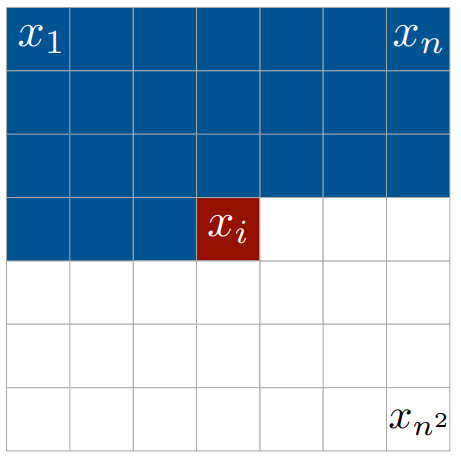
\includegraphics[width=0.35\textwidth]{images/Generative Networks/PixelRNN.png}
   \caption{Bestimmung von $\hat{p}(x)$ mit PixelRNNs \cite{pixelRNN}}
   \label{fig:pixelRNN}
\end{figure}

Um die beschriebene Abhängigkeit des momentan generierten Pixels zu allen bisher generierten Pixel umsetzen zu können, besitzen \acp{PixelRNN} eine Art \emph{Erinnerung}. Bisher wurden in dieser Arbeit nur sogenannte \emph{Feedforward} Netze behandelt, bei denen der Informationsfluss stets in eine Richtung erfolgt. Nämlich vom Eingang des Netzes zum Ausgang. Es existieren auch \emph{Recurrent Neural Networks}. Sie werden besonders zur Verarbeitung von natürlicher Sprache eingesetzt \emph(engl.: natural language processing). Abbildung \ref{fig:RNN} bildet hierfür eine beispielhafte Darstellung.

\begin{figure}[H]
   \centering
   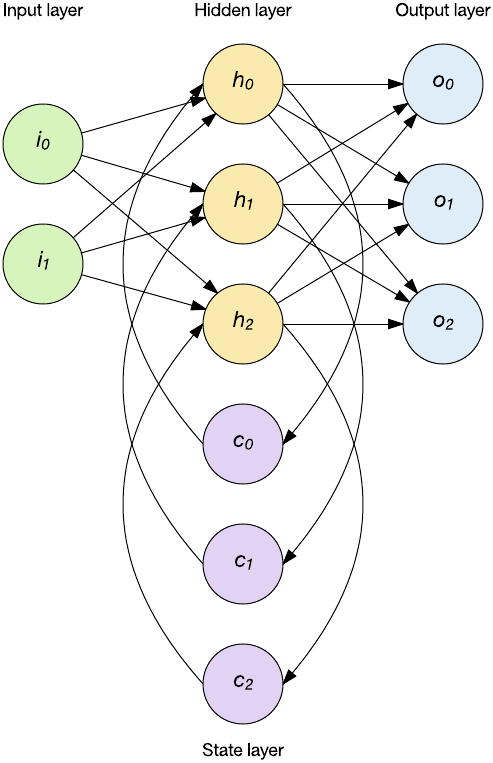
\includegraphics[width=0.4\textwidth]{images/Generative Networks/RNN.png}
   \caption{Darstellung eines Recurrent Neural Networks \cite{ibmRNN}}
   \label{fig:RNN}
\end{figure}

In Recurrent Neural Networks spielen die \emph{Zustände} eines Netzes eine besondere Rolle. Ein Zustand wird durch die Eingangs- und Ausgangswerte aller Neuronen zu einem gegebenen Zeitpunkt beschrieben. In \acp{PixelRNN} ist der Zustand des Netzes für den Pixel $x_{2}$ abhängig von dem Zustand des Netzes für $x_{1}$. Um solche Beziehungen darstellen zu können, besitzt das beispielhaft abgebildete Netz die Neuronen $c_{0}$ bis $c_{2}$, die den vorherigen Wert eines Neurons rekursiv auf seinen Eingang zurückführen. Somit wird der vorherige Zustand des neuronalen Netzes als zusätzlicher Eingang für die Berechnungen genutzt. \acp{PixelRNN} nutzen eine besondere Form der Recurrent Neural Networks. Sie arbeiten mit sogenannter \emph{Long Short-term Memory}. Dadurch soll das Problem behoben werden, dass in klassischen Recurrent Neural Networks weit in der Vergangenheit liegende Zustände nur noch einen geringen Einfluss auf den momentanen Zustand haben. \cite{generativeModelsSurvey}

Da die durch ein \ac{PixelRNN} umgesetzte Verteilung $\hat{p}(x)$ direkt erfassbar ist, wird ihnen nachgesagt, dass die Performanz solcher Netze gut evaluiert werden kann. Es gilt als vergleichsweise leicht, für solche Netze Metriken zur Messung der Performanz umzusetzen. Ein grundlegender Nachteil von \acp{PixelRNN} ist, dass die Generierung sequenziell erfolgt. Es ist in dem beschriebenen Verfahren nicht möglich, mehrere Pixel parallel zu generieren, da der Wert eines Pixels von denen aller vorher generierten Pixel abhängig ist. Dies verlangsamt die Generierung, da keine Parallelisierung möglich ist. \cite{generativeModelsSurvey}

Es existieren auch sogenannte \emph{PixelCNNs}, bei denen sich die Generierung stets nur auf bestimmte Bildbereiche konzentriert. Diese Bildbereiche können parallel zueinander sequenziell berechnet werden. Die Parallelisierung ist jedoch nur während des Trainings des Netzwerks oder während der Evaluation von $\hat{p}(x)$ für gegebene Bilder möglich. Die Bildgenerierung erfolgt auch hier, analog zu \acp{PixelRNN}, vollständig sequenziell. \cite{pixelRNN}

\subsection{Variational Autoencoder}

%In dieser Studienarbeit sollen \acp{GAN} zur Generierung künstlicher Bilder von Straßenschildern eingesetzt %werden. Dies ist jedoch nicht die einzige Möglichkeit, wie mittels \acp{KNN} künstliche Bilder erzeugt werden %können. In diesem Kapitel werden daher weitere Methoden vorgestellt, die ebenfalls dazu eingesetzt werden können.

%Eines der bisher genannten Beispiele für \acp{KNN} ist die Umsetzung eines Katzenklassifikators. Diese sogenannten %diskriminativen Modelle setzen grundlegend folgende Wahrscheinlichkeitsfunktion um:
%\begin{equation}
%   p(y|x)
%\end{equation}
%Bei einem Eingang $x$ soll das Modell die Wahscheinlichkeit für jeden Ausgang $y$ bestimmen. Zeigt man einem %Katzenklassifikator ein Bild auf dem keine Katze zu sehen ist, so soll $p(\mathrm{Katze}|x)$ gering sein. Die %Wahrscheinlichkeiten einer Wahrscheinlichkeitsverteilung müssen zusammen den Wert \emph{eins} ergeben, wodurch im %Umkehrschluss der Ausgang $p(\mathrm{KeineKatze}|x)$ eine hohe Wahrscheinlichkeit liefert. Um diese Verteilung %erlernen zu können, ist Supervised Learning notwendig.

%Generative Netze besitzen eine andere Aufgabe. Sie sollen neue Verteilungen generieren. Diese Verteilungen sollen %möglichst ähnlich der Verteilung sein, auf die das Modell trainiert wurde. Das Modell bestimmt, wie wahrscheinlich %es ist, dass ein gegebenes $x$ aus der Verteilung stammt. Konkret bezogen auf den Kontext dieser Studienarbeit: %Gibt man dem generativen Modell ein Bild, soll es bestimmen, wie wahrscheinlich es ist, dass dies ein real %aufgenommenes Foto eines Straßenschildes ist. Es wird folgende Wahrscheinlichkeitsfunktion umgesetzt:
%\begin{equation}
%   p(x)
%\end{equation}
%Wobei $p(x)$ als die Wahrscheinlichkeit interpretiert werden kann, dass ein gegebenes $x$ aus der Verteilung der %Trainingsdaten stammt.


%\subsection{Boltzmann Maschinen}
%\subsection{Deep Belief Netzwerke}